\chapter{\large Método para la Integración de Datos Basada en Ontologías}


\pagestyle{fancy}
\lhead{}
\chead{}
\rhead{Capítulo 2: Método para la integración de datos basada en ontologías}
\lfoot{}
\cfoot{}
\rfoot{\thepage}
\renewcommand{\headrulewidth}{0.4pt}
%\renewcommand{\footrulewidth}{0.4pt}
 \vspace{-1cm}

\section{Paradigma utilizado en el desarrollo del método}
La investigación en la disciplina de sistemas de información (SI) se caracteriza por dos paradigmas: las ciencias del comportamiento y las ciencias del diseño \citep{Hevner:2004:DSI:2017212.2017217}. El primer paradigma persigue el desarrollo y verificación de teorías que expliquen o pronostiquen el comportamiento humano u organizacional. El paradigma de las ciencias del diseño tiene como fin la creación de innovaciones que definan ideas prácticas, capacidades tecnológicas y productos a través de los cuales puede lograrse el análisis, diseño, implementación, gestión y uso de sistemas de información de manera efectiva y eficiente \citep{Denning:1997:NSC:253671.253755}. Un SI es un sistema basado en computadoras que ayuda a la gestión y uso de la información en una organización o entre varias organizaciones \citep{GarciaNoguera2009}. Analizando la naturaleza del problema tratado en esta investigación y la relación entre su campo de acción (el mecanismo para integrar datos relativos al Control de Autoridades en la aplicación informática AUCTORITAS) y la disciplina de SI, el desarrollo de la solución se concibió y ejecutó bajo el paradigma de las ciencias del diseño.

Las ciencias del diseño crean y evalúan artefactos orientados a mejorar y entender el comportamiento de los sistemas de información, estos artefactos pueden ser constructos, modelos, métodos e instanciaciones \citep{March:1995:DNS:1700865.1700867}. Los constructos pertenecen al vocabulario conceptual de un dominio y son empleados por los modelos para representar una situación del mundo real en términos del diseño de un problema y su espacio de solución \citep{Simon:1996:SA:237774}. La búsqueda dentro de ese espacio de solución es guiada por métodos, los cuales pueden ser algoritmos matemáticos, descripciones textuales del proceso de búsqueda o combinaciones de ambas \citep{Hevner:2004:DSI:2017212.2017217}. Las instanciaciones demuestran la viabilidad de implementar los métodos y modelos, a la vez que facilitan la evaluación concreta del artefacto que representan.

La presente investigación fue desarrollada según el proceso definido por \cite{Peffers2006} para las investigaciones en ciencias del diseño. Este proceso propone seis actividades secuenciales: identificación del problema y motivación, objetivos de la solución, diseño y desarrollo, demostración, evaluación y comunicación. Los resultados de la primera y segunda actividad fueron expresados en la introducción de este documento. El diseño y desarrollo incluye determinar las funcionalidades deseadas del artefacto y su arquitectura para luego crear el artefacto en cuestión. Los elementos esenciales que debe poseer una aplicación informática para el OBDA/OBDI se sintetizan en el subepígrafe \ref{Acceso e Integración de Datos Basado en Ontologías}. Los artefactos
creados serán descritos en los epígrafes siguientes, mientras que la demostración de su eficacia en la solución del problema, así como la observación y medición de su desempeño relativos a las actividades cuatro y cinco del proceso serán expuestas en el Capítulo \ref{Capítulo 3}. Como evidencia de la comunicación a otros investigadores del problema abordado en la investigación y su relevancia, el artefacto creado, su utilidad y su efectividad, se encuentran artículos publicados en revistas y trabajos presentados en eventos por el autor de esta investigación.

El método propuesto para la Integración de Datos Basada en Ontologías se denomina OntoIntegra. Este método describe el proceso para la integración de los datos almacenados en fuentes de datos estructuralmente heterogéneas en una respuesta conceptualmente homogénea, a partir de la instanciación de una ontología creada para la OBDI. El método se basa en los constructos: consulta sintáctica y instancia de una ontología.

\textbf{Definición 2.1.1} \textit{Una consulta sintáctica es la secuencia textual de instrucciones que permite recuperar información almacenada en al menos una fuente de datos.}

\textbf{Definición 2.1.2} \textit{Sea una ontología compuesta por una parte conceptual (T-Box) y una parte asercional (A-Box). Se denomina instancia de la ontología a su parte asercional.}

\section{OntoIntegra. Aspectos generales}
El aporte teórico fundamental de esta investigación es un método para la integración semántica de datos almacenados en fuentes estructuralmente heterogéneas. La figura \ref{fig: metodoOntoIntegra} ilustra el método propuesto, denominado OntoIntegra. Este método describe la obtención de información conceptualmente integrada a través de cinco pasos fundamentales:

\begin{enumerate}
\item Análisis estructural de cada fuente de datos.
\item Análisis semántico de la información almacenada en cada fuente de datos.
\item Instanciación de la ontología para OBDI.
\item Publicación de la instancia de la ontología creada.
\item Consumo por una aplicación informática de la instancia de la ontología creada.
\end{enumerate}

\begin{figure}
\begin{center}
	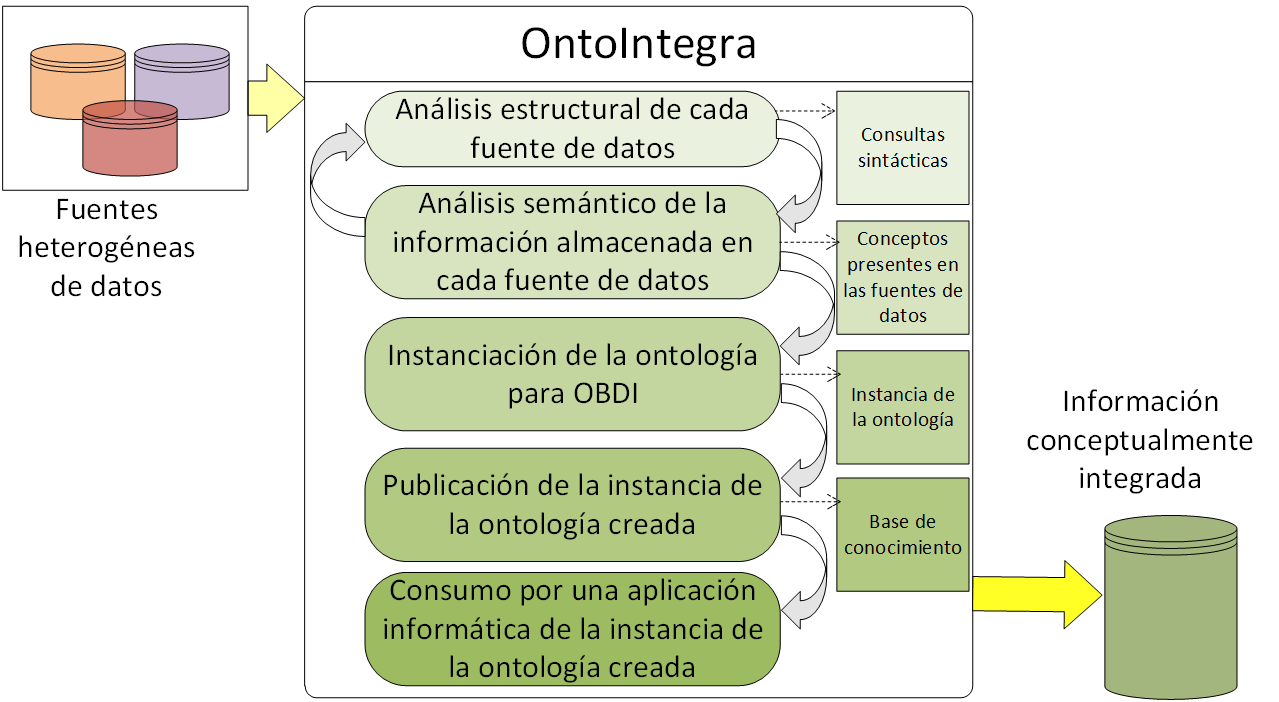
\includegraphics[width=0.8\textwidth]{img/Metodo_OntoIntegra.png}
\end{center}
\caption{Esquema representativo del método OntoIntegra}
\label{fig: metodoOntoIntegra}
\end{figure}

\section{Análisis estructural de cada fuente de datos}

El análisis estructural de cada fuente de datos tiene como objetivo identificar la forma en que se encuentran estructurados los datos a recuperar, formulando la consulta sintáctica adecuada a este proceso. En este paso interviene un Experto del dominio, el cual es una persona que conoce en detalle la estructura de los datos gestionados por la fuente de datos en cuestión. En el caso de las bases de datos relacionales, el ``Lenguaje de Consultas Estructurado'' (``Structured Query Language'' - SQL, por sus siglas de acuerdo al término en idioma inglés) constituye el estándar para la recuperación de datos \citep{Eisenberg:1999:SFK:309844.310075}. Este tipo de bases de datos se ha utilizado durante más de dos décadas \citep{BUCKLES1993660,Hristidis2002670,10.1007/978-981-10-8276-4_22}, por lo que gran parte de los datos almacenados a nivel mundial se encuentran sobre el modelo relacional.

Las bases de datos no relacionales, incluyendo las jerárquicas, orientadas a grafos y orientadas a objetos existen desde finales de la década de 1960 \citep{Leavitt2010}. Con el surgimiento y desarrollo de la Web 3.0, las bases de datos orientadas a grafos que soportan el modelo de datos RDF han ganado popularidad \citep{Zaki2017,BRISABOA2017106}. El lenguaje ``Protocolo SPARQL y Lenguaje de Consulta RDF'' (``SPARQL Protocol and RDF Query Language'' - SPARQL, por sus siglas de acuerdo al término en idioma inglés) es la recomendación del ``Consorcio de la World Wide Web'' (``World Wide Web Consortium'' - W3C, por sus siglas de acuerdo al término en idioma inglés) para la consulta sobre grafos RDF \citep{W3CSPARQLWorkingGroup2013}.

Cada vez son más los servicios que se publican en la Web usando REST \citep{Pautasso2014}. El estilo de arquitectura REST enfatiza la escalabilidad de las interacciones entre los componentes de las aplicaciones informáticas y promueve la reutilización de los componentes reduciendo su acoplamiento \citep{Pautasso2014}. Resulta posible considerar aplicaciones externas que exponen sus datos a través de REST como fuentes de datos. En este caso, el análisis estructural de la fuente de datos se centraría en la estructura sintáctica que debe poseer la petición a formular para extraer los datos a integrar.

\section{Análisis semántico de la información almacenada en cada fuente de datos}

El análisis semántico de la información almacenada en cada fuente de datos pretende determinar los conceptos contenidos en las mismas cuyos datos asociados se desean recuperar. En este paso interviene un Experto del dominio y un Ingeniero de conocimiento. El Ingeniero de conocimiento tiene la función de traducir los elementos presentes en una fuente de datos a conceptos comprensibles por un usuario externo.

En este paso un Usuario de conceptualización requiere ciertos conceptos sobre un dominio en específico, esta petición se la realiza a un Experto del dominio. El Experto del dominio determina exactamente qué elementos del dominio son los que necesita el Usuario de conceptualización y se lo informa al Ingeniero de conocimiento. El Ingeniero de conocimiento modela conceptualmente los elementos recibidos en términos conocidos por el Usuario de conceptualización y retorna la conceptualización elaborada. Este proceso se ilustra en la figura \ref{fig: conceptsExtraction}.

Para formalizar la conceptualización elaborada se decidió desarrollar la ontología que se describe en \ref{onto:hdrm}.\\

\begin{minipage}{\textwidth}
$Concept \equiv Thing \sqcap \exists mappedTo.Literal \sqcap =1 mappedTo \sqcap \exists type.Literal \sqcap =1 type \sqcap \forall name.String$ \\
$Connection \equiv Thing \sqcap \exists endpoint.Literal \sqcap =1 endpoint \sqcap \forall user.String \sqcap \forall password.String $ \\
$Datasource \equiv Thing \sqcap \exists composedBy.Concept \sqcap \exists has.Connection \sqcap =1 has \sqcap type.Literal \sqcap =1 type$ \\
\captionof{figure}{T-Box de la ontología desarrollada}
\label{onto:hdrm}
\end{minipage}


\begin{figure}
\begin{center}
	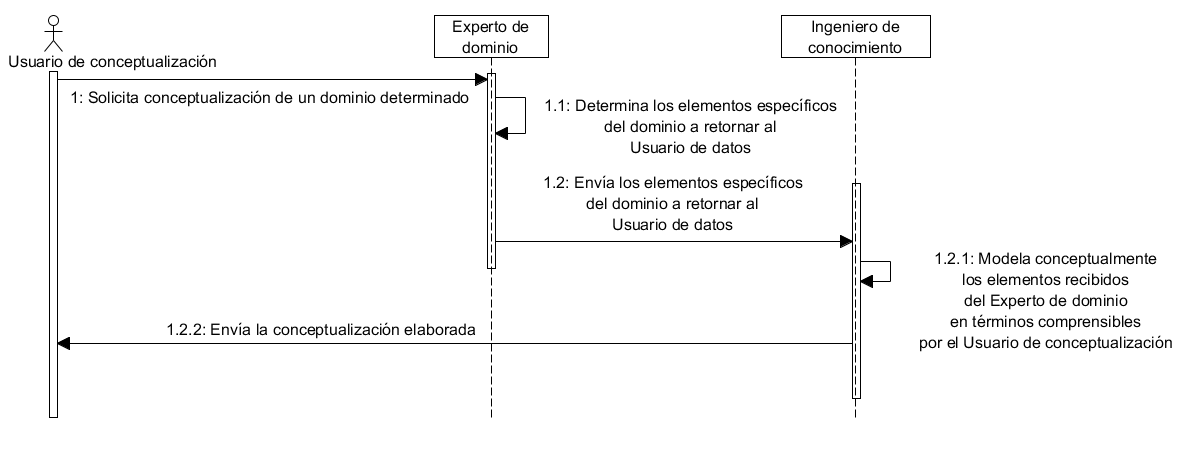
\includegraphics[width=0.8\textwidth]{img/conceptsExtraction.png}
\end{center}
\caption{Secuencia realizada en el paso Análisis semántico de la información almacenada en cada fuente de datos}
\label{fig: conceptsExtraction}
\end{figure}

\section{Instanciación de la ontología para la integración de datos}

La instanciación de la ontología para OBDI consiste en la representación de los conceptos identificados en el paso anterior acorde a la terminología definida por la ontología seleccionada. Según \cite{Calvanese2017} los elementos básicos que debe poseer una ontología diseñada con el propósito de permitir la OBDI son los definidos en la ontología \ref{onto:elementosBasicosOntologiaOBDI}.

\begin{equation}
Concepto \equiv Thing \sqcap \exists mapeo.Literal
\label{onto:elementosBasicosOntologiaOBDI}
\end{equation}

\section{Publicación de la instancia de la ontología creada}

La publicación de la instancia de la ontología creada se refiere a la carga en un almacén de tripletas RDF de la instancia creada.

\section{Consumo por una aplicación informática de la instancia de la ontología creada}

El consumo por una aplicación informática de la instancia de la ontología creada procura, a partir de la definición terminológica de la ontología, obtener su instanciación y utilizarla para recuperar los datos requeridos.







